%% Outline
% 1. Navigation is important problem
% 1.5 Traditionally addressed by mapping during exploration and path
%      planning during exploitation.
% 2. End to end learning algorithms have shown promise to take over
%      mapping and path
% 3. We do not know how these algorithms work. There has been work in computer vision that shows the learning on neural network based methods can be learning totally different kind of patterns from what we would expect.
% 4.1 We find that it is not remembering the map it is being trained on
% 4.2 We find that no path planning is  happening only, memorizing and regeneration of the sequence of steps. However, it is not 

% 1. Navigation is important problem
% 1.5 Traditionally addressed by mapping during exploration and path
%      planning during exploitation.
Navigation remains a fundamental problem in mobile robotics and artificial intelligence (\cite{SmChIJRR1986,ElCOMPUTER1980}).
The problem is classically addressed by separating the eventual task of navigation into exploration and exploitation. 
In exploration stage, the environment is represented as some kind of \emph{map}. 
In exploitation stage, the map is used to \emph{plan a path} to a given destination based on some optimality criterion. 
% VD: SLAM is just the exploration part. I think we should avoid introducing SLAM here.
% VD: why do we need to mention autonomous driving industry
 %This classical approach, traditionally called SLAM (Simultaneous Localization and Mapping), constitutes an entire subfield of robotics whose successes include the birthing of the autonomous driving industry. 
% SLAM however, possesses its own limitations.
This classical approach has been quite successful in navigation using variety of sensors. However, navigation in generic unstructured environments, especially with texture-less \cite{YaSoKaIROS2016}, transparent and reflective surfaces \cite{lai2011large}, remains a challenge.
% VD: ``subtly different'' Too generic of a claim
%Algorithms, especially those centered in vision, lack performance invariance often failing to extend results to environments that are subtly different from the ones they were trained on.
%As a simple example, state-of-the-art monucular SLAM methods fail when confronted with textureless environments.
% Moreover, in many application the mapping in full metric detail is unnecessary, which has prompted researchers to non-metric maps like topological maps \cite{beeson2010factoring}. However, with the decisions regarding 
% Furthermore, the decision about the required mapping details depends upon the end task of path planning, hence requires difficult decisions about the encoding of mapping data structures.


More recently, end-to-end navigation methods---methods that attempt to  
solve the navigation problem without breaking it down into separate parts of mapping and path-planning---have gained traction.
%
% 2. End to end learning algorithms have shown promise to take over
%      mapping and path-planning
With the recent advances of Deep Reinforcement Learning (DRL), these end-to-end navigation methods, like \cite{MnBaMiICML2016,SiHuMaNATURE2016,LePaKrISER2017,MiPaViICLR2017,OhChSiICML2016}, forego decisions about the details that are required in the intermediate step of mapping.
The potential for simpler yet capable methods is rich; for example, agents thus trained can potentially optimize the amount of map information that is required to perform the navigation task.
One such work, \cite{MiPaViICLR2017}, has demonstrated algorithms that are able to explore and find goals in complex environments utilizing only the monocular first-person view.
%Of significance is the fact that these agents upon finding the goal within a previously seen environment, are able to navigate to it faster in subsquent explorations implying that agents are able to learn to exploit map structures in the execution of learned navigational tasks. 

\begin{figure}
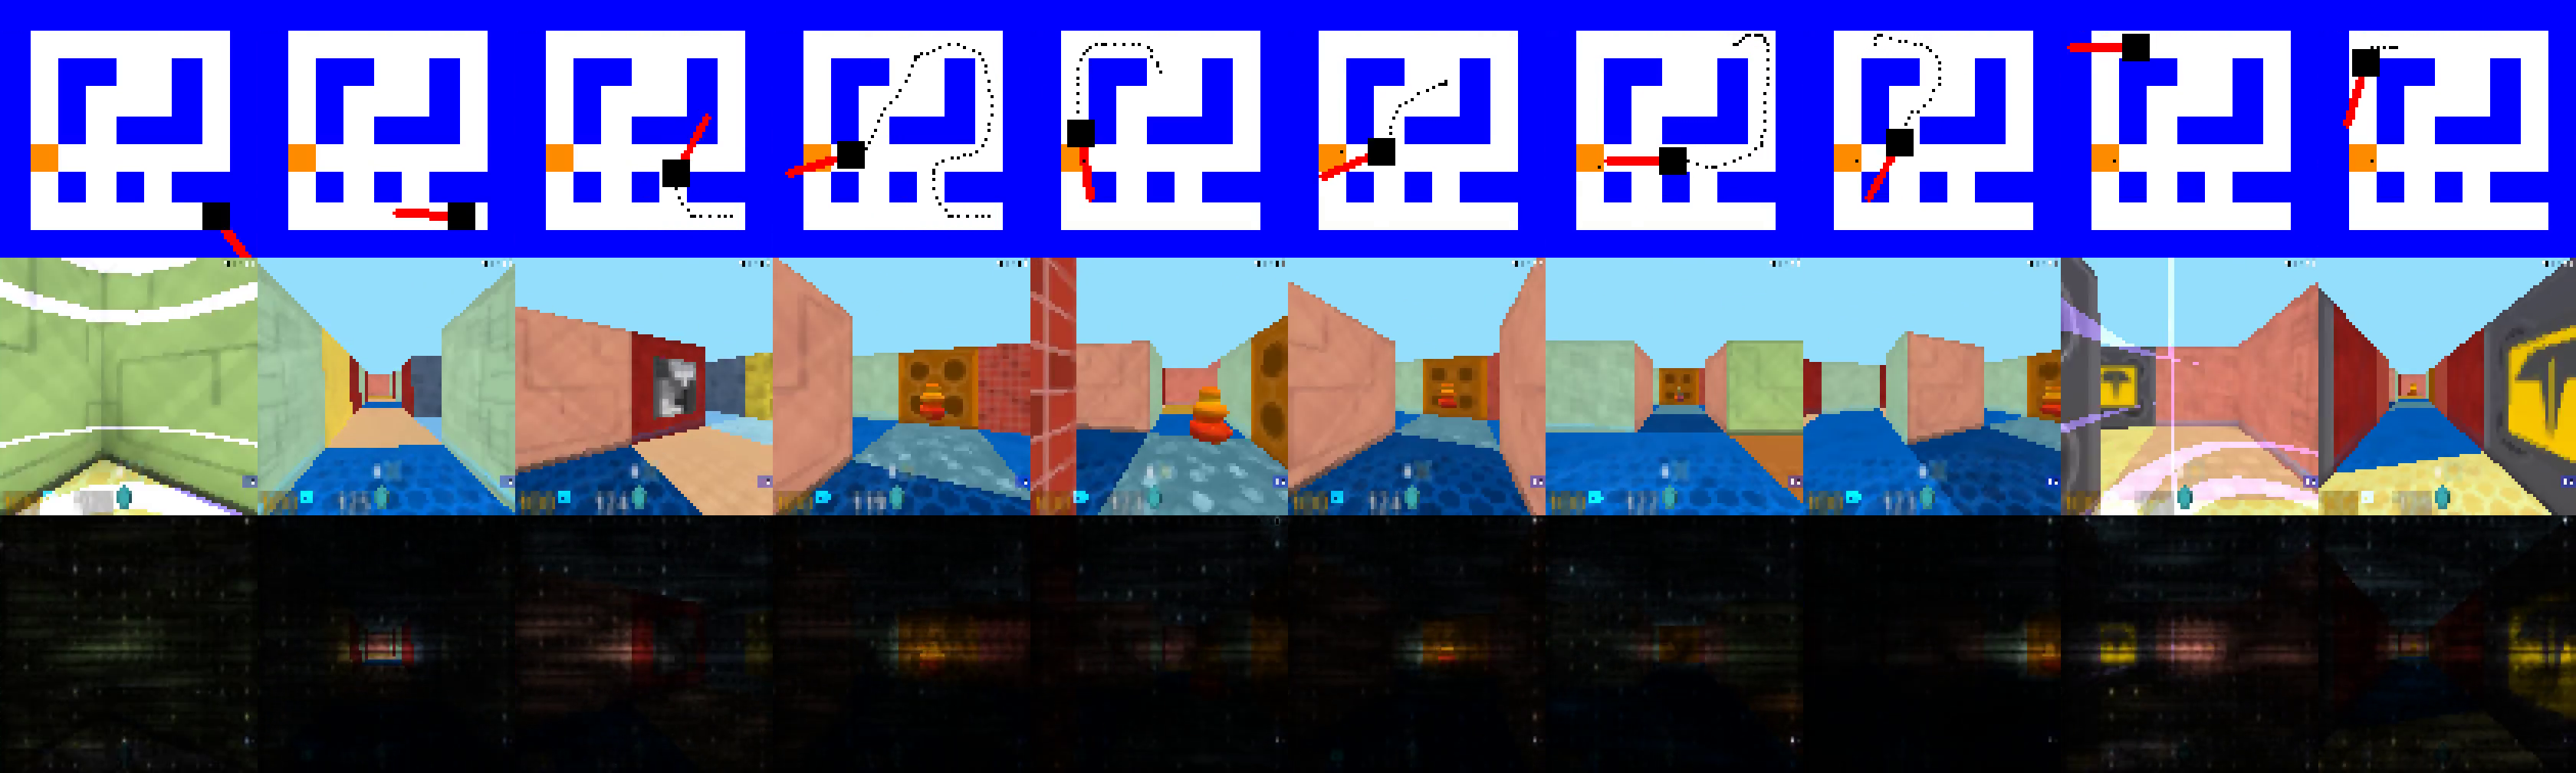
\includegraphics[width=\textwidth,trim=0 336pt 0 0,clip]{./exp-results/training-09x09-0127-on-0127.png}%
\caption{
Snapshots of the path taken by the agent while evaluating algorithm on map ID 127.
The top row shows the top view of the robot moving through the maze along with goal location in orange, second row shows the first person which is the only input available to the agent (except reward).}
\label{fig:training-qualitative}
\end{figure}

% 3. We do not know how these algorithms work. There has been work in computer vision that shows the learning on neural network based methods can be learning totally different kind of patterns from what we would expect.
Despite such potential advances, DRL based navigation remains a relatively unexplored field with its own set of limitations. 
The black-box nature of these methods make them hard to study and the patterns captured by the methods are not well understood. 
% VD: This is not the limitation of DRL algorithms
%Their exists no comprehensive set of experiments that answer how and when these algorithms perform well and how their performance differs based on variations in the training and testing conditions. 
% VD: This is a detail and is repeated in next paragraphs
% It is also unknown how well these algorithms generalize especially to previously unseen worlds.
Recent work in analyzing neural networks have shown that such object detection methods can be easily fooled by introducing noise that is imperceptible to humans (\cite{NgYoClCVPR2015}). 
This makes it even more important to analyze these DRL methods across a wide variety of experiments to understand their strengths and weaknesses.

% 4.1 We find that it is not remembering the map it is being trained on
% 4.2 We find that no path planning is  happening only, memorizing and regeneration of the sequence of steps. However, it is not 

% Prior setup
In this work, we build on \cite{MiPaViICLR2017} and analyze their methods across hundreds of maps with increasing difficulty levels. 
% VD: Cutting down unncessary sentences
% VD: No need to tell the license and name of the environment
%Our setup is similar, utilizing the same simulation environment, Deepmind Lab \cite{BeLeTeARXIV2016}.
We setup the environment as a randomly generated map as shown in Fig~\ref{fig:training-qualitative}, with an agent and a goal.
The agent is provided only with the first-person view and is tasked to find the goal maximum number of times within a fixed episode length.
We train and evaluate the algorithms with increasingly difficulty.
In the easiest stage, we keep the goal location, spawn location and map same during training and testing.
We call this experiment as \emph{static goal, static spawn, and static map}.
To increase the difficulty, we randomize one of spawn location, goal location and maps untill all three are random.
We discuss the design of experiments in Section~\ref{sec:navtasks} with more detail.
%We randomly genereate our mazes wherein the agent and goal are both statically and randomly spawned across experiments. 

\cite{MiPaViICLR2017} train and evaluate their algorithms with random goal, random spawn, and static maze and show that algorithm able to exploit the knowledge goal location at evaluation time to maximize reward.
However, this result is shown to be successful only on one map making the repeatability of the results questionable.
It is also unclear whether these results generalize to unseen maps.

Even though separating training and testing sets is standard practice in machine learning, to the best of our knowledge, we are the first work to evaluate any DRL based navigation method on maps with unseen structure.
We expand on \cite{MiPaViICLR2017} analysis to address above limitations and ask the question whether DRL based algorithms such as \NavAiiiCDiDiiL{} perform any mapping followed by shortest path planning.
We find no evidence of mapping in the cases when algorithms are evaluated on unseen maps and no evidence of optimal path planning even in cases when the map is same and only goal is randomized.

We also compute attention-maps for these agents to understand the kind of features used in the context of their navigation.
We find that the agents discard most of the image information, focusing attention on a small band in the middle of the image except for a few frames close to junctions where the attention is distributed evenly throughout the image.

These findings are the results on training and testing on multiple maps that were randomly chosen from a set of 1100 randomly generated maps.
We provide thorough and clear summaries of our data to substantiate these findings as well as individual maps and results to explain them carefully.
Unlike \cite{MiPaViICLR2017}, we will make our code and data available after the blind review process is over.

% Explained earlier
% % Systematic experiments
% To address this lacks of information about these agent's navigational abilities, we systematically expand upon \cite{MiPaViICLR2017}'s analysis by evaluate these agents and  metrics on a comprehensive set of randomly generated maps with differing training and testing conditions of increasing complexity. 
% In particular, we move from deterministic setups wherein the agents are trained on environments containing fixed spawn points, fixed goal locations and coincident training/testing maps to  much more complex cases involving random spawn points, random goal locations and diverged training and testing sets. 
% In particular, we quantitavely evaluate our trained models to test their map-exploitation abilitiesacross these differing setups and observe agents are unable to transfer this ability to the unseen worlds.
% Instead we observe that the agent's preferred path to the goal is just as an artifact of its initialized location and rotation and hypothesize that the agents are learning a correspondence between local sequences of frames and actions that lead to the goal.

% More contributions


